\chapter{\IfLanguageName{dutch}{Stand van zaken}{State of the art}}%
\label{ch:stand-van-zaken}

\section{Tekstvereenvoudiging}

Eerst moet er een technologische fundering gelegd worden over de basisconcepten en verschillende soorten van tekstvereenvoudiging. Tekstvereenvoudiging is het proces waarin het technisch leesniveau en/of woordgebruik van een geschreven tekst wordt verminderd. Zo mag de vereenvoudiging geen invloed hebben op de betekenis van de kerninhoud. Het langlopende onderzoek van Advaith Siddharthan is met meer dan 140 citaties een goed vertrekpunt voor dit onderzoek. Volgens \autocite{Siddharthan2014} bestaat een complete vereenvoudiging van een tekst uit precies vier transformaties. Binnen machinaal leren (ML) is tekstvereenvoudiging een zijtak van natuurlijke taalverwerking. % Daarnaast is tekstvereenvoudiging een taalbewerking dat geautomatiseerd kan worden.

\subsection{Natural Language Processing}

Natural Language Processing (NLP) of natuurlijke taalverwerking is een brede term die zich richt op het verwerken en analyseren van menselijke taal door computers en andere technologieën. Het omvat verschillende technieken, zoals tekstanalyse, taalherkenning en -generatie, spraakherkenning en -synthese, en semantische analyse. Computers zijn in staat om op een menselijke manier te communiceren en begrijpen wat er wordt gezegd. \textcite{Sohom2019} haalt de volgende begrippen aan.

\begin{itemize}
	\item \textbf{Tokenisatie} splitst de stam of basisvorm van woorden in een tekst. Gebruikelijk zetten ontwikkelaars deze stap in om een woordenschat voor een taalmodel op te bouwen. Bij tokenisatie wordt er geen rekening gehouden met de betekenis achter ieder woord.
	\item \textbf{Lemmatiseren} in NLP bouwt verder op \textit{stemming}, maar de betekenis van ieder woord wordt in acht genomen. Voor het lemmatiseren bestaan er Nederlandstalige modellen, waaronder JohnSnow\footnote{https://nlp.johnsnowlabs.com/2020/05/03/lemma\_nl.html}. Bij \textbf{omgekeerd lemmatiseren} wordt er een afgeleide achterhaald vanuit de stam. Bijvoorbeeld voor het werkwoord 'zijn' zou dit 'is', 'was' of 'ben' zijn. Voor zelfstandige naamwoorden, zoals 'hond', is dit dan enkelvoud of meervoud.
	\item Bij een \textbf{parsing}-fase wordt er een label aan ieder woord of zinsdeel toegekend. Voorbeelden van labels zijn zelfstandig naamwoord, bijwoord, werkwoord, bijzin of stopwoord. Het herkennen van zinsdelen wordt \textit{chunking} genoemd. Parsing heeft een dubbelzinnigheidsprobleem, want een 'plant' staat niet gelijk aan de vervoeging van werkwoord 'planten'.
\end{itemize}

\subsubsection{Sequence Labeling}

Volgens \textcite{Eisenstein2019} is \textit{sequence labeling} essentieel tot het achterhalen van de structuur van een tekst met \textit{supervised learning}. Elk woord in een tekst of zin wordt geclassificeerd met behulp van specifieke labels, zoals bijvoorbeeld een Part of Speech (PoS) label of een Named Entity Recognition (NER) label. De structuur van de tekst wordt achterhaald en informatie en patronen kunnen uit de tekst worden gehaald. \textcite{Jurafsky2014} haalt PoS- en NER-labeling verder aan in hun boek. Terwijl POS-tagging zich richt op grammaticale categorieën van woorden, richt NER-labeling zich op het identificeren van specifieke entiteiten in tekst. 

\begin{itemize}
	\item Bij \textbf{POS-tagging} worden de woorden in een zin geanalyseerd en krijgt elk woord een grammaticale categorie of een deel van de rede toegewezen, zoals zelfstandig naamwoord, werkwoord, bijvoeglijk naamwoord of bijwoord. POS-tagging helpt volgens \textcite{Jurafsky2014} bij het identificeren van de syntactische structuur van een zin. Dit is volgens de onderzoeker handig voor taken zoals parsing en machinevertaling. Dit wordt aanschouwelijk gemaakt op \ref{fig:pos}
	\item Aan de andere kant houdt \textbf{NER-labeling} zich bezig met het herkennen en classificeren van \textit{named entities} in een zin, zoals namen van personen, organisaties, locaties, data, enzovoort. NER-labeling wordt volgens \textcite{Jurafsky2014} gebruikt om specifieke informatie uit tekst te halen, zoals het identificeren van de namen van personen, plaatsen of bedrijven die in nieuwsartikelen worden genoemd, of het extraheren van belangrijke data of getallen uit financiële rapporten. Dit wordt aanschouwelijk gemaakt \ref{fig:ner}. \textcite{Li2018} haalt vier technieken aan waarop NER-labeling kan gebeuren:
	\begin{itemize}
		\item \textit{Dictionary-based} systemen waarbij een dictionary een verzameling van de woordenschat bijhoudt. Hierop wordt \textit{basic string matching} toegepast.
		\item \textit{Rule-based} systemen met een vooraf gekregen verzameling van regels voor het ophalen van informatie. Het toewijzen gebeurt met patronen, of met de context van een woord.
		\item \textit{ML-based} modellen trainen eerst op geannoteerde tekstdocumenten, vervolgens gebruikt het getrainede model deze annotaties.
		\item \textit{Deep-learning} of DL-modellen mappen de invoerdata aan een niet-lineaire representatie. De complexe modellen maken het mogelijk om niet voor de hand liggende relaties uit te pluizen, wat het de sterkste van de vier opties maakt.
	\end{itemize}
	Daarnaast haalt \textcite{Li2018} modellen aan om een pipeline voor NER-labeling mogelijk te maken. Spacy heeft deze functie ingebouwd. Standford NER-tagger is een tool die samen met het NLTK-pakket werkt.
\end{itemize}

\begin{figure}
	\begin{center}
		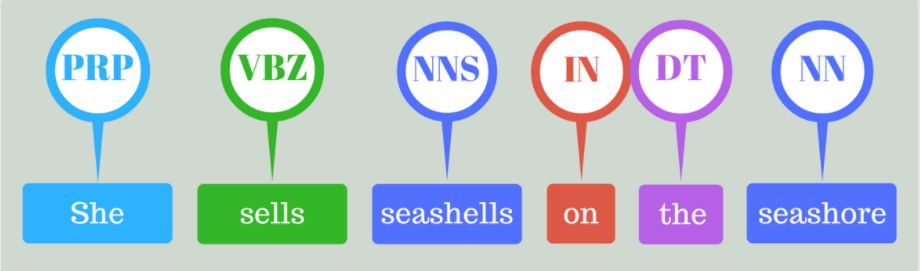
\includegraphics[width=10cm]{img/poslabeling.png}
	\end{center}
	\caption{Voorbeeld van PoS-labeling op de Engelstalige zin "She sells seashells on the seashore". Afbeelding van \textcite{Bilisci2021} }
	\label{fig:pos}
\end{figure}

\begin{figure}
	\begin{center}
		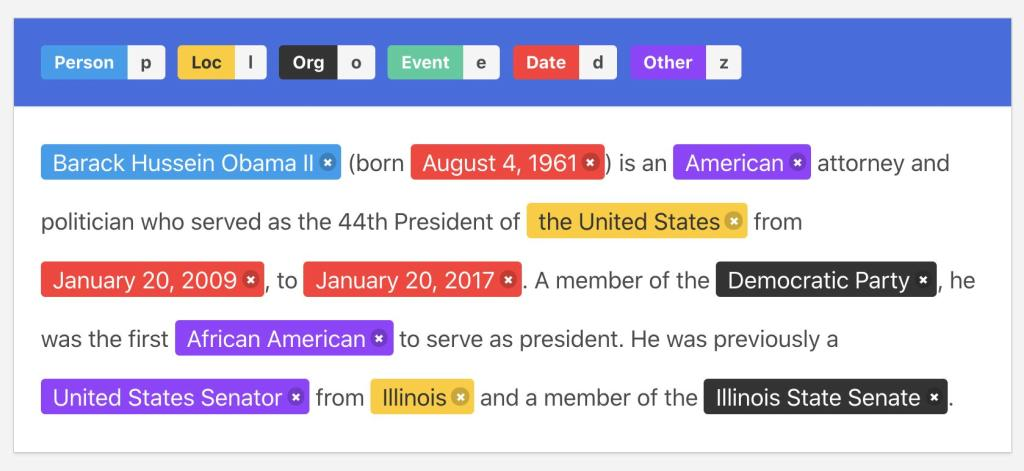
\includegraphics[width=10cm]{img/nerlabeling.jpg}
	\end{center}
	\caption{Voorbeeld van sequence labeling op de Engelstalige zin "She sells seashells on the seashore". Afbeelding van \textcite{Bilisci2021} }
	\label{fig:ner}
\end{figure}

\section{De verschillende soorten tekstvereenvoudiging}

Tekstvereenvoudiging bestaat uit vier soorten transformaties: lexicale, syntactische en semantische vereenvoudiging en samenvatten.

\begin{figure}
	\begin{center}
			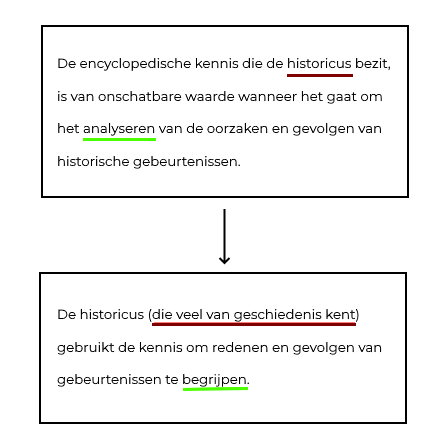
\includegraphics[width=5cm]{img/voorbeeld-manuele-vereenvoudiging.png}
	\end{center}
	\caption{Voorbeeld van manuele tekstvereenvoudiging. Oorspronkelijke tekst uit Historia 5 bron toe te voegen}
\end{figure}

\subsection{Lexicale vereenvoudiging}

% todo bron
Bij lexicale vereenvoudiging worden complexe woorden vervangen door eenvoudigere synoniemen. Bijvoorbeeld, het woord 'adhesief' kan worden vervangen door 'klevend'. De zinsstructuur verandert niet en er is garantie dat de kerninhoud en benadrukking hetzelfde blijft. Het doel van lexicale vereenvoudiging is om de moeilijkheidsgraad van de woordenschat in een zin of tekst te verlagen. Dit is, volgens het aantal onderzoeken, de meest gekende vorm van vereenvoudiging en een noodzakelijke stap bij het vereenvoudigen van een tekst. Voor prevalente domeinen, zoals de onderwijs-, medische en financiële sector, zijn er onderzoeken vrij beschikbaar. 

In de medische sector haalt \textcite{Kandula2010} twee manieren aan om lexicale vereenvoudiging mogelijk te maken, namelijk het vervangen door een synoniem en het aanmaken of genereren van extra uitleg. Zij bouwden verder op een vorig onderzoek van \textcite{Zeng2005}.

\subsection{Syntactische vereenvoudiging}

Syntactische vereenvoudiging transformeert de grammatica en zinsstructuur van een tekst om de complexiteit van een zin te verlagen. Bijvoorbeeld, twee afzonderlijke zinnen kunnen worden samengevoegd tot één eenvoudigere zin. Syntactische vereenvoudiging richt zich op het verminderen van complexe of onduidelijke zinsconstructies, terwijl de inhoud en betekenis van de tekst behouden blijft. Dergelijke transformaties zijn het vereenvoudigen van de syntax of door de zinnen korter te maken. Zinnen worden toegankelijker, zonder de kerninhoud of relevante inhoud te verliezen.

Het vereenvoudigen van medische journalen wordt besproken in het onderzoek van \textcite{Kandula2010}. Zij ontwikkelden een toepassing om medische informatie te vereenvoudigen met beschikbare biomedische bronnen, door syntactische vereenvoudiging op zinniveau toe te passen. Zinnen met meer dan 10 woorden worden als complex beschouwd en worden verwerkt door drie modules. Op het einde van deze vereenvoudiging kan de oorspronkelijke zin ongewijzigd worden behouden of vervangen worden door twee of meer kortere zinnen. De architectuur van het model omvat drie onderdelen: een \textit{Part of Speech (PoS) Tagger}, een \textit{Grammar Simplifier} en een \textit{Output Validator}. 

\begin{itemize}
	\item Voor de \textit{PoS Tagger}-fase gebruikten \textcite{Kandula2010} beschikbare functies uit het open-source pakket OpenNLP\footnote{https://opennlp.apache.org/}.
	\item De \textit{Grammar Simplifier} module splitst de lange zin in twee of meer kortere zinnen door POS-patronen te identificeren en een set transformatieregels toe te passen.
	\item De \textit{Output Validator} module controleert de output van de Grammar Simplifier op grammatica en leesbaarheid. Er zijn drie condities:
\end{itemize}  

% De toepassing werd getest met vier leesbaarheidsmetrieken en een "cloze"-test op verschillende soorten medische documenten, en liet verbeteringen zien in alle metingen. De verbeteringen waren echter relatief klein en er is meer uitgebreide gebruikerstesten nodig voor een betere validatie van het hulpmiddel. De resultaten lieten zien dat het hulpmiddel verbeterd was ten opzichte van eerdere versies. Er is verder werk nodig om de cohesiemeting te verbeteren en de methode voor het genereren van uitleg, waaronder het identificeren van geschikte verbindingswoorden en bronnen voor het genereren van betekenisvolle uitleg.

% todo probleemstelling van lexicaal vereenvoudigen

\subsection{Conceptuele of semantische vereenvoudiging}

Conceptuele vereenvoudiging lost dit probleem op. Theoretische kennis hierover is schaars, maar \textcite{Siddharthan2006} bestudeerde dit concept verder. Dit type vereenvoudiging betreft het opdelen van complexe concepten in eenvoudigere delen, het gebruik van duidelijke en bondige taal en het vermijden van technische jargon en abstracte uitdrukkingen. Het doel is om de inhoud begrijpelijker te maken, zonder dat hierbij de betekenis of nauwkeurigheid wordt aangetast. \textcite{Siddharthan2006} noemt deze transformatie een vorm van elaboratie of het uiteenzetten van een begrip.

\subsection{Semantische vereenvoudiging}

Semantisch vereenvoudigen is volgens \textcite{Siddharthan2006} de inhoud of betekenis van een tekst aanpassen om het begrijpelijker te maken voor een doelgroep. Zo wordt er meer uitleg of voorbeelden gegeven, of dat niet-relevante delen van de tekst worden weggelaten. 

\subsection{Tekstvereenvoudiging automatiseren}

Geautomatiseerde tekstvereenvoudiging is geen nieuw concept. Volgens onderzoeken van \textcite{Canning2000, Siddharthan2006} waren de eerste aanpakken op geautomatiseerde tekstvereenvoudiging gebouwd op rule-based modellen. Deze modellen bewerken de syntax door zinnen te splitsen, te verwijderen of de volgorde van de zinnen in een tekst aan te passen. Lexicale vereenvoudiging kwam hier niet aan de pas. Enkel bij recentere onderzoeken van \textcite{Coster2011, Bulte2018} werd het duidelijk hoe lexicale en syntactische vereenvoudiging gecombineerd kon worden.

\subsection{Combineren tot het geheel van tekstvereenvoudiging}

Het onderzoek van \textcite{DeBelder2010} richt zich op tekstvereenvoudiging voor kinderen. De doelgroep ligt echter jonger dan deze casus, maar het onderzoek haalt aan hoe de onderzoekers een methode opzetten voor lexicale en syntactische vereenvoudiging.

Een onderzoek van \textcite{Bulte2018} ging met dit concept aan de slag. Het resultaat van hun onderzoek was een \textit{pipeline} ontworpen om moeilijke woordenschat naar simpele synoniemen te vervangen. Eerst ging de tekstinhoud door een \textit{preprocessing}-fase, samen met het uitvoeren van WSE. Daarna werd de moeilijkheidsgraad van ieder token overlopen. De moeilijkheidsgraad is gebaseerd op hoe vaak een woord voorkomt in SONAR500\footnote{https://taalmaterialen.ivdnt.org/download/tstc-sonar-corpus/} een corpus met eenvoudige Nederlandstalige woorden. Synoniemen werden teruggevonden met Cornetto\footnote{https://github.com/emsrc/pycornetto}, een lexicale databank met Nederlandstalige woorden. Hiervoor gebruikten de onderzoekers een \textit{reverse lemmatization} fase. Lexicale vereenvoudiging is ingewikkeld wanneer er geen eenvoudigere synoniemen zijn. In dat geval blijft een moeilijk woord voor wat het is.

\section{Samenvatten}

% Probleem met de voorbije fasen

Teksten vereenvoudigen met lexicale, conceptuele en/of syntactische vereenvoudiging biedt geen garantie dat de tekstinhoud korter zal worden. Bij deze drie soorten wordt er enkel binnen een zin gekeken, zo wordt er geen rekening gehouden met de zinnen die daarop voorafgaan of volgen.

% Zinnen opsplitsen leidt volgens \textcite{Siddharthan2014} vaak uit tot langere zinnen, omdat de zinsbouw per opsplitsing vanaf nul moet worden opgebouwd. 

% TODO https://files.eric.ed.gov/fulltext/ED490073.pdf --> bron !!!

% Informatieve, indicatieve en kritische samenvattingen

Teksten machinaal samenvatten is geen nieuw concept. Het onderzoek van \textcite{Hahn2000} bevat vele citaties en een uitgangspunt om te vertrekken hoe teksten automatisch kunnen worden samengevat. Zij halen twee aanpakken hoe een machine een tekst kan samenvatten: extractief en abstractief. Verder reikt \textcite{Hahn2000} drie soorten samenvattingen aan:

\begin{itemize}
	\item Informatieve samenvattingen vervangen de oorspronkelijke tekst. Alles wat de lezer nodig heeft, dus hoofd- en bijzaken, zijn betrokken in de samengevatte tekst.
	\item Indicatieve samenvattingen behouden enkel een tekst met links die een lezer doorverwijzen naar andere bronnen. 
	\item Kritische samenvattingen of \textit{reviews} bestaan uit de kerninhoud van de oorspronkelijke tekst en een opiniestuk over die specifieke kerninhoud.
\end{itemize}

% Generiek en gebruikersgerichte samenvatting

Verder haalt \textcite{Hahn2000} ook het onderscheid tussen een generieke en een gebruikersgerichte samenvatting. Een generieke samenvatting staat niet stil bij speciale noden of interesses van de eindgebruiker. Daarnaast houdt een gebruikersgerichte samenvatting wel rekening met sleutelwoorden of thema's in een tekst. \textcite{Hahn2000} haalt aan dat technologieën zoals full-text-search en gepersonaliseerd informatiefiltering het belang van gebruikersgerichte samenvatting naar voor duwen.

\textcite{Hahn2000} omschrijft de architectuur van een samenvattingssysteem aan de hand van drie fases. Allereerst wordt de brontekst geanalyseerd. Daarna worden de \textit{salient points} of kernpunten in een tekst aangeduid. Deze punten zijn zinnen of tokens. Ten slotte worden de punten samengevoegd tot één uitvoertekst. De nadruk is verschillend per samenvattingsmethode.

\subsection{Extractief samenvatten}

Bij deze vorm worden de belangrijkste zinnen gemarkeerd en vervolgens opnieuw neergeschreven.  Dit is het equivalent van handmatig zinnen te fluoriseren en vervolgens op een blanco papier neerschrijven. Het nadeel hiervan is dat de uitvoertekst niet samenhangend zal zijn na het samenvatten. Dit maakt de tekst minder aangenaam om te lezen. \textcite{Verma2020} onderzocht de verschillende manieren waarop een tekst op een extractieve manier kan worden samengevat. Zij halen drie grote componenten aan, namelijk:

\begin{itemize}
	\item Graph-based
	\item Maximal Marginal Relevance
	\item Meta-heuristic-based
\end{itemize}

% todo Bij deze vorm worden de belangrijkste zinnen gemarkeerd en vervolgens opnieuw neergeschreven.  Dit is het equivalent van handmatig zinnen te fluoriseren en vervolgens op een blanco papier neerschrijven. Het nadeel hiervan is dat de uitvoertekst niet samenhangend zal zijn na het samenvatten. Dit maakt de tekst minder aangenaam om te lezen.
\subsubsection{Graafgebaseerd extractief samenvatten}

Graafgebaseerd extractief samenvatten is een techniek die een document voorstelt als een graaf, waarbij de knopen zinnen voorstellen en bogen de relatie tussen de zinnen voorstellen. Deze algoritmen achterhalen de belangrijkste zinnen in de graaf. Bijvoorbeeld kan het PageRank-algoritme, dat vaak wordt gebruikt voor het rangschikken van webpagina's in zoekmachines, worden gebruikt om de zinnen in de grafiek te rangschikken op basis van hun belangrijkheid.

\textcite{Parveen2015} raadt een graafgebaseerd systeem aan voor \textit{unsupervised learning}. Belangrijke zinnen worden bepaald met een lokaal minimum, alsook wordt redundantie vermeden. Deze methode blijkt goed te werken bij het ophalen van samenvattingen uit zowel lange wetenschappelijke artikelen als korte nieuwsartikelen. Daarnaast vermeldt \textcite{Parveen2015} ook dat het systeem altijd beter presteert wanneer coherentie wordt opgenomen en wanneer het wordt gecombineerd met positionele informatie. In toekomstig werk is \textcite{Parveen2015} van plan om meer taalkundige informatie in de entiteitsgrafiek op te nemen en beoordelingen van domeinexperts te verkrijgen om te zien of de redactiesamenvattingen als gouden samenvattingen kunnen worden gebruikt voor evaluatie.

\textcite{AbdelSalam2022} voerden een vergelijkend onderzoek uit rond SqueezeBERT en BERT. Met behulp van de compacte architectuur van SqueezeBERT kan een samenvatter worden gemaakt en ingezet voor real-time samenvatting. Dit is volgens de onderzoeker een interessant alternatief voor de originele BERT-base samenvatter, die meer dan 120 miljoen trainbare parameters heeft. In vergelijking heeft de voorgestelde SqueezeBERT slechts ongeveer 62 miljoen parameters, terwijl het samenvattingsprestatieniveau nog steeds boven de 90\% van het BERT-baseline model blijft. Uit de experimenten van \textcite{AbdelSalam2022} blijkt dat de SqueezeBERT-samenvatter een goed alternatief is om een samenvatter te trainen met bijna de helft van de grootte van het originele model met minimale afbreuk in de samenvattingsprestaties. Daarnaast blijkt uit het onderzoek dat het gebruik van efficiënte netwerken geïnspireerd door \textit{computer-vision literature}, zoals \textit{grouped convolutional layers}, de NLP downstream taken kan verbeteren.  \textcite{AbdelSalam2022} haalt verder aan dat er potentie is voor een productieversie van een SqueezeBERT-samenvatter, die minder parameters heeft dan DistilBERT met ongeveer 20\% en dezelfde ROUGE-1 score behoudt, terwijl het iets hogere ROUGE-2 en ROUGE-L scores behaalt. Hoewel de SqueezeBERT en DistilBERT iets lagere scores produceren in vergelijking met het BERT-baseline model, heeft SqueezeBERT als voordeel dat het minder trainingstijd en minder parameters heeft dan het baseline model met ~48,44\%. 


% https://www.mdpi.com/2078-2489/13/2/67

\subsubsection{Maximal Marginal Relevance}

De traditionele extractieve samenvattingssystemen bouwen verder op de architectuur dat \textcite{Carbonell1998} ontworp. Hun ontworpen architectuur gebruikt een maximaal marginale relevantiescore of MMR. Deze architectuur houdt rekening met de diversiteit en de relevantie van de gemarkeerde zinnen. De relevantie van een zin wordt bepaald door de mate waarin het de belangrijkste informatie overbrengt van de tekst waarvan het afkomstig is. Om diversiteit te waarborgen, wordt er gekeken naar de mate waarin de geselecteerde zinnen verschillen van de eerder geselecteerde zinnen in de samenvatting. Met andere woorden, als er een zin is die erg relevant is, maar qua inhoud te veel overlapt met de eerder geselecteerde zinnen, dan heeft deze minder kans om geselecteerd te worden in de samenvatting. Deze score kan doorgaans berekend worden met KeyBERT\footnote{https://maartengr.github.io/KeyBERT/api/mmr.html}.

Extractief samenvatten met de MMR-methode is de methode bij uitstek voor ML-toepassingen. Onderzoekers bouwden verder op dit principe. In \textcite{McDonald2007} stelt de onderzoeker voor om de gulzige zoekalgoritme van MMR te vervangen door een globaal optimale formulering, waarbij het MMR-framework wordt uitgedrukt als een knapzakprobleem en er een integer lineair programmering (ILP) solver kan worden gebruikt om de functie te maximaliseren. De MMR-methode hield voordien enkel rekening met relevantie en diversiteit, maar niet met de optimale combinatie van zinnnen die in een samenvatting moet worden opgenomen. Deze aanpak vereist echter meer rekenkracht en tijd dan de standaard MMR-methode, maar het experiment van \textcite{McDonald2007} haalde wel aan dat dit leidde tot betere resultaten. \textcite{Lin2010} evolueerde het oorspronkelijke MMR-algoritme. Bij de evaluatie van deze architectuur benadrukte zij betere resultaten. 

\subsubsection{Metaheuristiek-gebaseerd}

Metaheuristieke samenvatting maakt gebruik van metaheuristieke optimalisatie-algoritmen zoals genetische algoritmen, \textit{simulated annealing} of zwermoptimalisatie om de belangrijkste zinnen in een tekst te achterhalen. Volgens \textcite{Verma2020} \textcite{Premjith2015} worden deze algoritmen gebruikt om te zoeken naar de beste combinatie van zinnen die de belangrijkste informatie in de tekst kunnen vertegenwoordigen. De fitnessfunctie die wordt gebruikt in metaheuristische samenvattingsalgoritmen kan gebaseerd zijn op verschillende criteria, zoals zinslengte, zinsrelevantie en zinscoherentie.

Echter haalt het onderzoek van \textcite{Rani2021} aan dat een metaheuristieke methode bij het samenvatten van teksten vaak vastraakt in een lokaal optima. Zij benoemen het vastlopen in een lokaal optimum als een shortcoming. Daarboven halen ze aan dat metaheuristieke methoden geen \textit{steepness} of extremen op een \textit{search space behaviour} aanduiden. Dit betekent dat de voorgestelde methode een optimalisatiestrategie gebruikt die gebaseerd is op gradiënten om de convergentie aanzienlijk te versnellen. 

% gradienten: (een wiskundig concept dat de richting van de snelste toename aangeeft)
% convergentie: (het proces waarbij het algoritme naar de juiste oplossing toewerkt) -- Hierdoor wordt het algoritme efficiënter en sneller uitgevoerd.


\subsubsection{Experimenten over extractief samenvatten}
% \subsubsection{title}

% todo https://medium.com/jatana/unsupervised-text-summarization-using-sentence-embeddings-adb15ce83db1 --> voorbeeld van een pipeline

\textcite{McKeown1999} voerden experimenten uit op het extractief samenvatten van teksten. Zij achterhalen dat deze vorm vatbaar is op vooroordelen. Bij nieuwsartikelen wordt er geen rekening gehouden met vooroordelen van de auteur. De zinnen worden genomen zoals ze zijn. \textcite{Hahn2000} bouwde verder op dit experiment. Zij voerden een experiment uit met een mix van \textit{knowledge-rich} en \textit{knowledge-poor} methoden, met succesvolle resultaten tot gevolg.

De nadruk bij extractief samenvatten ligt in het kiezen van de \textit{salient text units}. Deze punten zijn typisch in de vorm van zinnen. Er is nood aan een manier om de lexicale en statistische relevantie van een zin te kunnen aanduiden. Hiervoor haalt \textcite{Hahn2000} twee manieren aan:

\begin{itemize}
	\item Met een lineair gewicht model. Iedere teksteenheid wordt gewogen op factoren zoals de \textit{location weight} en het aantal voorkomens.
	\item Een gewicht model op basis van de statistische opvallendheid van een eenheid. Zo wordt er rekening gehouden met de aanwezigheid van een woord in (sub)titels.
\end{itemize}

% resultaten lineair gewicht model
% resultaten statistische opvallendheid

\textcite{Nallapati2017} wilden de nauwkeurigheid van andere modellen overbruggen. Dit doen ze met \textit{SummaRuNNer}\footnote{https://github.com/hpzhao/SummaRuNNer}, een oplossing voor het extractief samenvatten van teksten met een neuraal netwerk. De toepassing werd opgebouwd met PyTorch in  en bestaat uit een combinatie van drie modellen: een recurrent neuraal netwerk, een convolutioneel recurrent neuraal netwerk en een \textit{hiërarchical attention network}.

\subsubsection{Programmeren}

\subsection{Abstractief samenvatten}

Kernzinnen achterhalen gebeurt met zes belangrijke features volgens \textcite{Khan2014}. Zij onderzochten de verschillende manieren om een tekst samen te vatten. Ze halen een semantische en een structuurgerichte aanpak aan.

Om een abstractieve samenvatting op te bouwen bestaan er verschillende modellen. Het Pegasus-model vloeide voort uit een onderzoek van \textcite{Zhang2020} over het afhandelen van \textit{gap-sentences} met pre-trained models voor samenvatting met NLP. Pegasus haalt kernzinnen uit een invoertekst en zal die zinnen vervolgens als één uitvoerzin uitschrijven. Dit model werd getrained en beoordeeld op samenvattingstaken zoals emails, patenten, rekeningen en ook wetenschappelijke artikelen. Hieronder een code-snippet van hoe een simpele abstractieve samenvatting kan worden gemaakt met Google Pegasus.

\begin{lstlisting}[language=Python]
def test return
\end{lstlisting}

\subsection{Conclusie}

De theoretische concepten om teksten te vereenvoudigen. Teksten kunnen op vier manieren worden vereenvoudigd, namelijk door 

\section{Onderzoeken rond dyslexie}

\subsection{Noden van een student dyslexie}

Vlaamse en Nederlandse onderzoeken wijzen uit dat gemiddeld 4\% van de Nederlandstalige bevolking een vorm van dyslexie heeft. De prevalentie van dyslexie is taalafhankelijk. China heeft volgens ... 1\% van de bevolking, terwijl het cijfer bij het Engels, een orthografisch inconsistente taal, drastisch hoger ligt. 

Dyslectische kinderen ondervinden een last bij het technisch lezen van een tekst. Het is geen checklist van 'kwalen' waaraan een scholier moet voldoen om dit te bezitten. Zo halen Ghesquière en de Stichting Dyslexie van Nederland samen drie verschillende criteria.

\begin{itemize}
	\item Het \textbf{achterstandscriterium} wijst aan dat er een ernstige lees- of spellingsachterstand is. 
	\item Het \textbf{hardnekkigheidscriterium} houdt in dat de lees- of spellingsachterstand het gevolg is van een moeizame automatisering van het lees- en spellingsproces. De leessnelheid vertraagt, terwijl het aantal lees- of spellingsfouten verhoogt terwijl een scholier complexe taken uitvoert.
	\item Het \textbf{exclusiviteitscriterium} volgens Ghesquière wijst erop dat lees- en spellingsstoornissen niet volledig verklaard worden door andere condities, zoals verstandelijke beperkingen, emotionele moeilijkheden of zintuiglijke beperkingen.
\end{itemize}

% todo bronnen

Bij de derde criterium moet er extra worden stilgestaan en staat parallel met dit onderzoek. Niet alle personen met dyslexie hebben dezelfde problemen en noden. Zo halen ... de volgende kenmerken aan die kunnen verschillen per individu.

\begin{itemize}
	\item De ernst of uigebreidheid van een stoornis.
	\item De gevolgen van een stoornis, zoals faalangst.
	\item De mate waarin iemand al dan niet kan compenseren.
	\item De secundaire kenmerken zoals problemen met werkhouden en structuur.
\end{itemize}

% todo bronnnen

Verder wijst ... aan dat de prevalentie van gecombineerde reken- en leesstoornissen hoger ligt, geschat op een 25 tot 50\%. De prevalentie van het voorkomen van spraak- en taalstoornissen ligt op 50 tot 80\%. ... onderzocht of kinderen met dyslexie als groep al dan niet problemen hebben met begrijpend lezen. Het onderzoek richtte zich op het achterhalen van een groepsprofiel en of dit profiel al dan niet overeenkomt met individuele profielen. Hier achterhaalden ze met een cross-sectioneel onderzoek hoe:

\begin{itemize}
	\item De handelingsgerichte opbouw en de analyse van het begrijpend leesprofiel: Een hulpverlener een beeld kan krijgen van de beheersting van leesstrategieën, zoals geheugen, verbaal begrip, interpretatie op meso- en macroniveau en extrapolatie.
	\item Het begrip van complextalige informatie in een tekst in kaart brengen. De lezer die al dan niet de context van een tekst beheerst. Dit aan de hand van het koppelen van de juiste betekenissen aan de juiste woorden en zinnen.
	\item Het interpretatieniveau van de lezer.
	\item Verbanden leggen met de gelezen informatie op een actieve niveau leggen, zoals bij causale of logische inferentievragen. 
	\item Categorale inferenties waar de lezer een begrip in een bepaald ordeningskader plaatst.
	\item Logische inferenties waarbij de voorkennis wordt opgeroepen en geïntegreerd tijdens het lezen van teksten. 
	\item Bij de anaforische inferenties wordt er gepolst naar het gebruik van antecedenten of anaforen. De schrijver haalt echter aan dat verwijswoorden nog steeds noodzakelijk zijn, want deze maken de tekst aangenamer om te lezen.
	\item Causale en anaforische inferenties zijn de belangrijkste interpretaties op paragraafniveau, omdat zij in veel teksten voorkomen.
	\item Om de denkrelatie uit te voeren, moeten meerdere elementen uit verschillende paragraven met elkaar in verband worden gebracht. Afhankelijk van de aard van de opdracht volstaat het om verbanden in een volledige tekst te leggen of tussen twee paragrafen te zetten. De lezer moet nog steeds in staat zijn om tekst te kunnen samenvatten of om de hoofdgedachte en het thema van een tekst aan te duiden.
	\item Een kind moet verder kunnen redeneren over de inhoud van een tekst, nadat de lezer een deel van de tekst of de volledige tekst heeft gelezen. 
\end{itemize}

Het onderzoek van VanVreckem2022 benadrukt dat therapeuten in de eerste plaats een beeld moeten krijgen van de beheersing van de belangrijkste leesstrategieën, zoals het onthouden van gelezen informatie en het verbaal begrip. Daarnaast is er een zicht nodig op de beheersing van de belangrijkste leesstrategieën bij begrijpend lezen. Het interpreteren op mesoniveau wijkt onderling sterk af. Om een behandelplan op maat van een client te  kunnen maken, moet een testleider een zicht hebben op de beheersing van de belangrijkste begrippen. Als tweede moet het onderzoek aantonen of een groep met een comorbide stoornis beter of slechter presteert voor spelling dan de geïsoleerde groep. Alsook of er een verschil was tussen de spellingvaardigheden voor bestaande woorden vergeleken met pseudowoorden. Alle woorden uit alle dictees sluiten aan bij de Vlaamse leerplannen, alsook alle spellingcategorieën werden opgenomen in het experiment. Ten slotte hield het experiment rekening met de structurele en linguïstische moeilijkheidsgraad van woorden.

\begin{itemize}
	\item Kinderen met dyslexie ondervinden minder problemen bij het spellen van pseudowoorden.
	\item Kinderen met dyslexie hebben meer problemen met de spelling van bestaande woorden, dan met de spelling van pseudowoorden.
\end{itemize}

Het onderzoek beklemtoont dat er nood is aan verregaande en geïndividualiseerde analyse, om zo een effectieve behandeling op maat te kunnen voorzien. Een standaardpakket oefeningen laten afwerken heeft geen zin, noch voor het lezen, noch voor het spellen, noch voor het rekenen. De gegeven instructies zijn even belangrijk. Op groepsniveau zijn er opmerkelijke verschillen voor het totale testresultaat en het leggen van relaties in een volledige tekst. Verder zijn er op individueel niveau grote verschillen bij het interpreteren op mesoniveau. Een zicht op de soort inferenties binnen deze categorie, zoals causale, logische en anaforische inferenties is nodig. 50 van de 60 kinderen heeft een ernstige achterstand voor spelling van bestaande woorden. Er waren géén verschillen tussen de spellingvaardigheden van de groep kinderen met geïsoleerde dyslexie, vergeleken met de groep met comorbide stoornissen. Een bijkomende stoornis heeft geen impact op de spellingprestaties van een kind. De ene persoon met dyslexie is de andere niet. De proefgroep uit het onderzoek toont aan hoe divers de verschijningsvorm van de stoornis dyslexie is, door de aanwezigheid van spelling- of leesproblemen.


\subsection{Tekstvereenvoudiging voor scholieren met dyslexie in het onderwijs}

Het onderzoek van ... haalt drie factoren aan dat scholieren met dyslexie kan helpen bij het lezen van teksten. Allereerst bevoordeelt een hoge woordfrequentie de leessnelheid van een scholier met dyslexie. Dit feit wordt ondersteund in meerdere onderzoeken (...). 


Het onderzoek van \textcite{Filipak2020} verzamelde de noodzakelijke leesproblemen voor deze casus. Zo haalt hij de volgende leesproblemen aan die kunnen voorkomen bij een scholier met dyslexie in het middelbaar onderwijs.

\begin{itemize}
	\item Langzame woordbenoeming
	\item Begripsproblemen
	\item Hardnekkig letter-voor-letter lezen
	\item Woordherkenning
	\item Visuele dysfunctie
	\item Letter- en klankvorming
\end{itemize}

\subsubsection{Langzame woordbenoeming}

Het correct spellen van pseudowoorden en regelmatig gespelde woorden is mogelijk via beheerste letterklankkoppelingen. Echter verloopt het automatiseren van moeilijke en nieuwe woorden stroef, met een trage woordbenoeming tot gevolgd. Lezers kunnen met dit leesprobleem veel woorden niet als één geheel herkennen. (...) raadt aan om pseudowoorden en het identificeren te oefenen als mogelijke hulp. De meeste schrijffouten komen voor in onregelmatig gespelde woorden waardoor een fonologische route die wel takt is, leidt tot het schrijven van 'gedaan' als 'guhdaan'.

% todo oplossing

\subsubsection{Begripsproblemen}

Typerende symptomen van ‘Deep Dyslexia’ is de verstoring van leesbegrip en het spreken in qua betekenis onbedoelde klanken, woorden en woordgroepen (parphasias). Bij ‘Deep dyslexia’ kan bos bijvoorbeeld gelezen worden als boom. Begripsproblemen bij het lezen kunnen goed visueel, met steun van film en afbeeldingen ondersteund worden, beter dan alleen via gedrukte woorden. Daarbij moet de lezer die het gedrukte woord wil ontcijferen, gebruik kunnen maken van bronnen van kennis op een hoger niveau: een grote woordenschat en een goed redeneervermogen. Schriftelijke expressie is uit den boze.

\begin{itemize}

	\item Hardnekkig letter-voor-letter lezen: Milene Bonte merkt op: wat wel typerend is voor ‘dyslexie’ is een minder optimale informatie-verwerking in visuele gebieden die belangrijk zijn voor letter- en woordherkenning. Ze haalt verder aan dat dit een gevolg is van een minder optimale leesontwikkeling en niet zozeer een oorzaak van dyslexie. Het visuele proces vindt plaats in de 'letterbox'\footnote{Het primaire visuele cortex van het brein}. Lezers zijn niet in staat woorden goed te lezen, zelfs niet met een langzame en spellende letter-klankroute. Lange woorden worden moeizaam gelezen en scholieren hebben de neiging om visueel gedesoriënteerde te raken. Er is verwarring over de richting van de letters.
	
	\item Woordherkenning: Onderzoeken waarbij de oogbewegingen van lezers worden gevolgd tonen aan dat een geoefende lezer bij vijftig tot tachtig procent van de woorden pauzeert. Hij moet zich op woorden fixeren om ze te kunnen zien en dat gaat heel snel. Gedurende deze zogenoemde saccade, een snelle beweging van de ogen die tot doel heeft een nieuw fixatiepunt te vinden, wordt het woordbeeld van de vorige woordfixatie onderdrukt, voordat een volgende woord wordt gefixeerd. Leesonderzoekers de Universiteit van Tel Aviv in Israël vonden in 2010 bijvoorbeeld een soort leesprobleem dat men ‘aandachts-dyslexie’ noemde, waarin kinderen letters correct identificeren, maar tijdens het lezen last hebben van verspringende letters tussen de woorden in de zinnen.[xiii] Dit is minder bij het lezen van woorden in lijsten dan met woorden in lopende tekst. [xiv] Denk aan het verschil in leesprestaties op de Drie-Minuten-Test (losse woorden lezen) en op de AVI -toets (tekstlezen). Zie ook in de breinafbeelding het gebied ‘Top-down attention and serial reading’. In een WISC-afname kan blijken dat de organisatie van de ruimtelijke waarneming redelijk is, maar dat een leerling zwakker is met doolhoven, plaatjes ordenen, onvolledige tekeningen, substitutie-taken en vooral met symboolverwerking. Dan kan er sprake zijn van een visueel en/of neuropsychologische dysfunctie dat ten grondslag ligt aan de moeite met lezen. Dan gaat het dus , nogmaals, niet om een fonologische dysfunctie.
	
	\item Visuele dysfunctie
	
	\item Letter- en klankverwarring: Verder gaat het om de verwisseling van de lettervolgorde, om letterweglatingen, letter-toevoegingen, letter-vervangingen, en het onherkenbaar verminken van woorden in dictees. En ook om de moeite met auditieve analyse en synthese. Veel kinderen kunnen deze leesfouten maken en dat is dan niet meteen fonologische dyslexie. [xviii]
\end{itemize}

% https://wij-leren.nl/leesproblemen-dyslexie-woordbenoeming-woordherkenning-begripsprobleem-deel-twee.php#_edn11


% \section{Voordelen van tekstvereenvoudiging}

% \textcite{Leopold2015} voerden een experiment uit om een leerstrategie te achterhalen bij het leren van wetenschappelijke teksten. Ze testen drie leermethoden: het markeren van zinnen, \textit{concept mapping} en het visualiseren van de tekst. Dit experiment werd uitgevoerd bij 51 scholieren van gemiddeld vijftien jaar en met een licht overwegend vrouwelijk publiek. Het experiment gaf geen inzicht over de leesbegaafdheid van een scholier. Als resultaat

% Improving students’ science text comprehension through metacognitive self-regulation when applying learning strategies

\section{Struikelblokken}

\subsection{Evaluatie van de toepassing}

\subsection{Datasets}

\subsection{Meaning distortion}

\subsection{Word Ambiguity}

Sequence Labeling voorziet labels aan tokens in een tekst. Homoniemen kunnen echter roet in het eten gooien, want . 

\subsection{Paternalisme}
De doelstelling van assisterende software is om gelijke kansen te bieden aan iedereen. Zoals eerder vermeld, zorgt tekstvereenvoudiging voor een simpelere syntax en woordenschat in een tekst. Volgens \textcite{Niemeijer2010} zijn de ethische overwegingen die samenhangen met tekstvereenvoudiging via implicaties voor assistieve technologie niet gemakkelijk te scheiden van de technologie die wordt gebruikt om het resultaat te bereiken. Ontwikkelaars moeten, volgens deze auteur, rekening houden met de doelgroep waarvoor ze een toepassing maken.

Het onderzoek van \textcite{Gooding2022} richtte zich op dit probleem. Ontwikkelaars moeten zich meer bewust worden van de behoeften en verwachtingen van de eindgebruiker bij het ontwikkelen van een tekstvereenvoudigingstoepassing. Haar onderzoek benadrukt de paternalistische en afhankelijke aard van assisterende toepassingen. Tekstvereenvoudiging omvat drie transformaties, maar de moeilijkheidsgraad is niet statisch. Een adaptieve tekstvereenvoudigingstoepassing moet de eindgebruiker een keuze aanbieden om aan te passen wat vereenvoudigd wordt, afhankelijk van zijn of haar specifieke behoeften.

% Xu bron
Volgens \textcite{Punardeep2020}, maken de meeste AI-toepassingen voor tekstvereenvoudiging gebruik van \textit{black-box} modellen. Een \textit{black-box} model maakt het onmogelijk om transparant te zijn over waarom bepaalde transformaties worden uitgevoerd, bijvoorbeeld het vervangen van een woord door een eenvoudiger synoniem. Het model kan dus niet aangeven waarom het juist dat woord heeft vervangen door dat specifieke synoniem. Deze AI-toepassingen vallen onder de categorie van \textit{supervised learning} en het model leert handelingen uit de data waarop het is getraind. Dit is echter problematisch, aangezien \textcite{Xu2015} benadrukt dat veel toepassingen voor tekstvereenvoudiging geen rekening houden met de doelgroep waarvoor ze zijn ontwikkeld.

Om dit probleem op te lossen, is het belangrijk om de eindgebruiker, in dit geval scholieren met dyslexie in het derde graad middelbaar onderwijs, de keuze te geven. Zoals beschreven in \textcite{Gooding2022}, zijn er verschillende mogelijkheden. Bijvoorbeeld, de eindgebruiker moet de mogelijkheid hebben om te kiezen welke synoniemen de tekst lexicaal zullen aanpassen. Een alternatieve aanpak voor syntactische vereenvoudiging is om de scholier zelf zinnen te laten markeren die moeilijk te begrijpen zijn, zodat het systeem alleen de door de eindgebruiker aangegeven zinnen vereenvoudigt.


\subsection{Problemen bij lexicale vereenvoudiging}

\begin{itemize}
	\item Acroniemen
	\item Homoniemen
\end{itemize}

\subsection{Problemen bij syntactische vereenvoudiging}

\begin{itemize}
	\item Kerninhoud verliezen
\end{itemize}

\section{Wetenschappelijke artikelen}

% https://goldbio.com/articles/article/how-to-read-and-understand-hard-scientific-papers
% https://www.science.org/content/article/how-seriously-read-scientific-paper
% https://journals.plos.org/plosone/article?id=10.1371/journal.pone.0189753

\section{Beschikbare software voor tekstvereenvoudiging}

\subsection{Toepassingen nu in het onderwijs beschikbaar}

\subsection{Online toepassingen}

\section{Prototype voor tekstvereenvoudiging}

% fasen aanhalen

\subsection{Lexicale vereenvoudiging}

\subsection{Syntactische vereenvoudiging}

\subsection{Samenvatten}

\section{Evaluatiemetrieken}

% Tip: Begin elk hoofdstuk met een paragraaf inleiding die beschrijft hoe
% dit hoofdstuk past binnen het geheel van de bachelorproef. Geef in het
% bijzonder aan wat de link is met het vorige en volgende hoofdstuk.

% Pas na deze inleidende paragraaf komt de eerste sectiehoofding.

% Dit hoofdstuk bevat je literatuurstudie. De inhoud gaat verder op de inleiding, maar zal het onderwerp van de bachelorproef *diepgaand* uitspitten. De bedoeling is dat de lezer na lezing van dit hoofdstuk helemaal op de hoogte is van de huidige stand van zaken (state-of-the-art) in het onderzoeksdomein. Iemand die niet vertrouwd is met het onderwerp, weet nu voldoende om de rest van het verhaal te kunnen volgen, zonder dat die er nog andere informatie moet over opzoeken \autocite{Pollefliet2011}.

% Je verwijst bij elke bewering die je doet, vakterm die je introduceert, enz.\ naar je bronnen. In \LaTeX{} kan dat met het commando \texttt{$\backslash${textcite\{\}}} of \texttt{$\backslash${autocite\{\}}}. Als argument van het commando geef je de ``sleutel'' van een ``record'' in een bibliografische databank in het Bib\LaTeX{}-formaat (een tekstbestand). Als je expliciet naar de auteur verwijst in de zin, gebruik je \texttt{$\backslash${}textcite\{\}}.
% Soms wil je de auteur niet expliciet vernoemen, dan gebruik je \texttt{$\backslash${}autocite\{\}}. In de volgende paragraaf een voorbeeld van elk.

% \textcite{Knuth1998} schreef een van de standaardwerken over sorteer- en zoekalgoritmen. Experten zijn het erover eens dat cloud computing een interessante opportuniteit vormen, zowel voor gebruikers als voor dienstverleners op vlak van informatietechnologie~\autocite{Creeger2009}.
